\chapter{Communication}
A communication system is desired for transporting the GoT data, calculated to coordinates on the computer, to the microcontroller, located on the vehicle. Furthermore a protocol handling packet transitions is necessary to implement on top of the communication system to be able to fulfil requirements set in \secref{Requirements}.

\section{OSI model}
The Open Systems Interconnection, OSI, model is a standard used to describe how information circulates in a network. Each layer describes a standardization of what should occur in the specific layer \cite{Microsoft}. The seven layers of the OSI model are illustrated in \tableref{tab:OSIModel}.

\begin{table}[H]\centering
\begin{tabular}{|p{1.5cm}|p{3cm}|}
\hline%-----------------------------------------------------------------------------------------------------------------
  \textbf{Layer} & \textbf{OSI} \\
\hline%-----------------------------------------------------------------------------------------------------------------
    7 &    Application      \\
\hline%-----------------------------------------------------------------------------------------------------------------
    6 &    Presentation      \\
\hline%-----------------------------------------------------------------------------------------------------------------
    5 &    Session       \\
\hline%-----------------------------------------------------------------------------------------------------------------
    4 &    Transport    \\
\hline%-----------------------------------------------------------------------------------------------------------------
    3 &   Network     \\
\hline%-----------------------------------------------------------------------------------------------------------------
    2 &   Data Link     \\
\hline%-----------------------------------------------------------------------------------------------------------------
    1 &    Physical     \\
\hline%-----------------------------------------------------------------------------------------------------------------
\end{tabular}
\caption{OSI model}
\label{tab:OSIModel}
\end{table}\vspace{-5mm}
Starting from the buttom, the Physical layer is the electrical/mechanical hardware layer. The layer handles bits and determines the communication medium, e.g. a copper cable or radio waves, and what is defined as a binary 0 and 1.\\The prototype utilizes two XBee modules, see \secref{Hardwarechoice}, one on the computer and one on the vehicle, for the lowest layers of communication. The XBee already implements this layer through the IEEE 802.15.4 protocol \cite{Xbee,IEEE812154}. It uses radio frequencies in the 2,4 \si{GHz} spectrum band.

The Data Link layer's functionality ensures physical addressing, error control when transferring data between nodes over the physical layer, and access control \cite{J.M.Network}. The Data Link layer is something the Xbee module also handles through IEEE 802.15.4, to check that it transmits bytes correctly and from and to which physical device it is transmitted \cite{IEEE812154}.

The Network layer's main functionality allows for the routing across a network with many nodes. This is not utilized in the prototype's protocol stack, since the communication is made only between two Xbees, i.e. two nodes.

The Transport layers handles packets and has the ability to assemble or disassemble them. An important part of the functionality of this layer is to ensure reliable transmission of data packages through error control, retransmission, or possibly through connection-oriented communication. For the prototype, a connectionless protocol is used, see \secref{sec:Protocol}.

The Session layer's role is to establish connections between two nodes. It is not needed in the prototype since a connectionless communication protocol is used.

The Presentation layer should define how payload data is arranged for the Application layer to use it. These two layers are already implemented through another prototype's functionality, i.e. the Route Control, see \secref{Finalprototype}, with the presentation being a simple set of two coordinates.

%Since the session is more overall version of network and the presentation layer transforms the code into something application layer can utilize for user interface. These application is not needed when communicating between the computer and the vehicle, since no user interaction is implemented and a one-way communication between two units is utilized. 

\section{Protocol}\label{sec:Protocol}
The main object for the communication system is to transmit the coordinates from the computer to the microcontroller. A transport layer protocol is created to ensure packets can be transmitted, received, i.e. the needed information can be extracted from the packet, and be able to identify erroneous packets.

A connectionless system is implemented, since it is one-way communication, from the computer to the microcontroller and retransmission not desired, since the vehicle is moving and a retransmission of a coordinate will cause a delay. Additionally, the sampling rate of the GoT system is 10 \si{Hz}, so transmitting the recently received coordinates would be sufficient. Therefore, erroneous packages are thrown away and acknowledgements are not utilized.

\subsection{Protocol Package Structure}
A package structure is desired for containing necessary information for addressing, decrypting and error handling. The protocol has a header which contains a start byte, a destination and the length of the package. The body of the package is the data and the tail is the checksum and the end byte. The package structure is illustrated in \tableref{CoorSetup}.

\begin{table}[H]\centering
\begin{tabular}{|>{\centering\arraybackslash}m{2cm}|>{\centering\arraybackslash}m{3cm}|>{\centering\arraybackslash}m{2cm}|>{\centering\arraybackslash}m{2cm}|>{\centering\arraybackslash}m{2cm}|>{\centering\arraybackslash}m{2cm}|}
\hline
Start Byte & Destination ID & length & Data & Checksum & End byte \\
\hline
\end{tabular}
\caption{The structure of a package}
\label{CoorSetup}
\end{table}

\subsubsection{Destination ID}
The Destination ID is to ensure packages, which is transmitted, is handled by the correct receiver. This way the transmitter can transmit to numerous receivers if multiple vehicles is utilized. The destination ID ensures the receivers can filter out packages not intended for them. The microcontroller has the destination ID 0000 0001. The length of the destination byte is set to one byte, so the destination can be read immediately when received.
\newpage
UDP, a connectionless protocol, utilizes a source, but in this case it is not necessary, since only one computer is transmitting, the receiver does not need to know where the package has been transmitted from. Even if more computers were utilized it would not be necessary as long as the package is marked with the destination ID, the receivers is able to read it. If retransmission was utilized, in case of erroneous packages, a source is necessary to have the ability to ask for a retransmission from the sender. Since retransmission is not utilized a source is not included in the package structure.

\subsubsection{Length}
The Length is utilized by the receiver. This will make it possible for the receiver to know the bit length of the package, and thereby know when the package should end. Each package created has the same length. The length is set to contain 7 bits, this can count up to $2^{7}-1 = 127$, which is sufficient.

\subsubsection{Data}
The data received from the GoT system consist of three coordinates (X,Y,Z), locating the position of the vehicle. Each of these coordinates can have a value from -9000 to 9000 (see \secref{GoTDescription}). To contain a number of this size, a 15 bit signed integer is utilized. Of the 15 bit 14 bit is utilized for the magnitude of the coordinate, which can have a value of 16385 ($2^{14}-1$). The last bit of the 15 bit is utilized to indicate if a coordinate is positive or negative, i.e. sign bit. The protocol is designed so the sign bit will be placed at the end of the 15 bit integer. As both the microcontroller and the computer utilizes little endians, there will not be a problem with the transmission of numbers. With little endians, the bit with the highest value will be located next to the sign bit and the bit with the lowest value is located at the beginning of the bit array. This will yield the bit array illustrated on \tableref{CoorSetup}.

\begin{table}[H]
\centering
\begin{tabular}{|>{\centering\arraybackslash}m{0.5cm}|>{\centering\arraybackslash}m{0.5cm}|>{\centering\arraybackslash}m{0.5cm}|>{\centering\arraybackslash}m{0.5cm}|>{\centering\arraybackslash}m{0.5cm}|>{\centering\arraybackslash}m{0.5cm}|>{\centering\arraybackslash}m{0.5cm}|>{\centering\arraybackslash}m{0.5cm}|>{\centering\arraybackslash}m{0.5cm}|>{\centering\arraybackslash}m{0.5cm}|>{\centering\arraybackslash}m{0.5cm}|>{\centering\arraybackslash}m{0.5cm}|>{\centering\arraybackslash}m{0.5cm}|>{\centering\arraybackslash}m{0.5cm}|>{\centering\arraybackslash}m{0.65cm}|}
\multicolumn{15}{c}{15 bits} \\
\hline
$2^0$ & $2^1$ & $2^2$ & $2^3$ & $2^4$ & $2^5$ & $2^6$ & $2^7$ & $2^8$ & $2^9$ & $2^{10}$ & $2^{11}$ & $2^{12}$ & $2^{13}$ & $+/-$ \\
\hline
\end{tabular}
\caption{Setup for the bit array, that contains one of the coordinate values.}
\label{CoorSetup}
\end{table}

The representation of the integer is called signed magnitude. Another representation that could be used is ones' complement. Here the number is inverted if the signed bit is true. But for an easier implementation on the computer, the signed magnitude is utilized. The code firsts checks if the number is positive or negative. If negative, the sign bit is set and the number is multiplied by minus one, this will yield the magnitude. The magnitude is then converted into a bit array. When converting back, it is only necessary to multiply the magnitude by minus one, if the sign bit is true.

\subsubsection{Checksum}
To ensure package data is received correctly, error handling is added to the protocol. A error handling which is utilized is a checksum. The way the checksum is calculated, is by splitting the header and the data up into pieces of equal size and then summing the pieces together. The summed bit array is then inverted and the remaining bit array is the checksum. 

there is 60 bit in the header and the data combined, i.e. 15 per coordinate, 8 for the destination and 7 for the length. these will be split up into three pieces of 20 bit. The related checksum consist of 20 bit. Combined, the header, data and checksum is 80 bit, which is equal to 10 bytes. In \tableref{ChecksumExp} an example of calculating a checksum is given.

\begin{table}[H]
\centering
\begin{tabular}{c c c c c c c c c c c}
   & Bit array  &     & Decimal &     & Bit 0-3 & Bit 4-7 & Bit 8-11 & Bit 12-15 & Bit 16-19 & Bit 20 \\
\hline
a) & Part 1     & $=$ & 123008  & $=$ & 0000 & 0001 & 0000 & 0111 & 1000 & \\
b) & Part 2     & $=$ & 351365  & $=$ & 1010 & 0001 & 0011 & 1010 & 1010 & \\
c) & Part 3     & $=$ & 729671  & $=$ & 1110 & 0010 & 0100 & 0100 & 1101 & \\
d) & Part 1+2+3 & $=$ & 1204044 & $=$ & 0011 & 0010 & 1111 & 1010 & 0100 & 1 \\
e) & Add carry  & $=$ & 155469  & $=$ & 1011 & 0010 & 1111 & 1010 & 0100 & \\
f) & Checksum   & $=$ & 893106  & $=$ & 0100 & 1101 & 0000 & 0101 & 1011 & \\
g) & Check      & $=$ & 1048575 & $=$ & 1111 & 1111 & 1111 & 1111 & 1111 & \\
\end{tabular}
\caption{The pieces consisting of the destination 1, length with the value of 96, and the data which is 4259, 7511 and -6418.}
\label{ChecksumExp}
\end{table}

The three pieces is added together, the destination, length and the data (see on line d). This produces a carry, since the checksum has the size of 20 bit. The carry is added to the beginning of the sum (line e). The generated sum is then inverted to yield a checksum (sees on line f).

When the receiver utilizes the checksum, it needs to check if the destination, length and data corresponds with the related checksum. The checksum is first added together with the three 20 bit pieces and, if there is any, the carry. If the outcome of the bit summation results in 20 bits which are true, then the package is received correctly. If not, the receiver will throw away the package. An error in the received package could be a bit inversion or some data not received by the receiver. 

A flaw when utilizing the created checksum, is that an error can cancelled out another error, and thereby make some errors undetectable. This can happen when the system adds the three pieces and the checksum together. An example, is if the first bit in piece number one is true and the first bit in piece number two is false. If both of these bits are shifted independently, so the bit from part one become false and the bit in part two true, the checksum can not detect the error. The likelihood for this to happen is very slim, as the errors first have to occur and then they have to be located a place where they cancel each other out. Having only 4 pieces of 20 bits, the likelihood of this happening is lesser than if the checksum was set to 10 bit. Since the addition occurs with 7 pieces of 10 bit. This would yield more bits with the same rank, so there would be a higher possibility for a bit cancelling each other out. This is a good argument for utilizing a larger checksum, even if it uses more space.

\subsubsection{Start and end byte}
As the computer transmits a package each time it receives coordinates from the GoT system, a queue of packages can appear in the microcontroller, if package handling is too slow. To not make the system able to differentiate packages from each other a start byte is added at the beginning of the package and an end byte at the end of the package. 

To find the start of a package the system will search for a start byte. When finding the start byte, it will read the destination, length, data and checksum and then look for a end byte. If the end byte is not found at that point, then the package is not received correctly and is thrown away. If the end byte is found, then system utilize the package and apply error handling on it. 

The start byte is set to 0000 1111. This is chosen to ensure the start byte does not have an identical value with another byte in the header. This is done to ensure no misunderstandings occurs. The end byte will come just before the next start byte. The value of the end byte is inverted compared to the start byte, this yields an end byte of 1111 0000.

The destination, length, data, checksum, start and end byte has been described, and a final package structure is illustrated in \tableref{PackageLook}

\begin{table}[H]
\centering
\begin{tabular}{|c|c|>{\centering\arraybackslash}m{0.3cm}|>{\centering\arraybackslash}m{0.3cm}|>{\centering\arraybackslash}m{0.3cm}|>{\centering\arraybackslash}m{0.3cm}|>{\centering\arraybackslash}m{0.3cm}|>{\centering\arraybackslash}m{0.3cm}|>{\centering\arraybackslash}m{0.3cm}|>{\centering\arraybackslash}m{0.3cm}|>{\centering\arraybackslash}m{0.3cm}|>{\centering\arraybackslash}m{0.3cm}|>{\centering\arraybackslash}m{0.3cm}|>{\centering\arraybackslash}m{0.3cm}|>{\centering\arraybackslash}m{0.3cm}|>{\centering\arraybackslash}m{0.3cm}|>{\centering\arraybackslash}m{0.3cm}|>{\centering\arraybackslash}m{0.3cm}|}
\hline
\multicolumn{2}{|c|}{Offsets} & \multicolumn{8}{c}{Byte 1} & \multicolumn{8}{|c|}{Byte 2} \\
\hline
\multicolumn{1}{|c}{Byte} & \multicolumn{1}{|c|}{Bit} & 0 & 1 & 2 & 3 & 4 & 5 & 6 & 7 & 8 & 9 & 10 & 11 & 12 & 13 & 14 & 15 \\
\hline
0 & 0 & \multicolumn{8}{c}{Start byte} & \multicolumn{8}{|c|}{Destination} \\
\hline
2 & 16 & \multicolumn{7}{c}{Length} & \multicolumn{9}{|c|}{X coordinate} \\
\hline
4 & 32 & \multicolumn{6}{c}{X coordinate} & \multicolumn{10}{|c|}{Y coordinate} \\
\hline
6 & 48 & \multicolumn{5}{c}{Y coordinate} & \multicolumn{11}{|c|}{Z coordinate} \\
\hline
8 & 64 & \multicolumn{4}{c}{Z coordinate} & \multicolumn{12}{|c|}{Checksum} \\
\hline
10 & 80 & \multicolumn{8}{c}{Checksum} & \multicolumn{8}{|c|}{End byte} \\
\hline
\end{tabular}
\caption{Illustration of a package, that will be send from the transmitter to the receiver.}
\label{PackageLook}
\end{table}\vspace{-5mm}
This yields a package with a length of 96 bit (12 byte). As the GoT system have a sampling frequency of 10 Hertz and each sample is converted to 12 bytes, the transfer speed for the Xbee have to be greater than 120 bytes per second, which it is \secref{Hardwarechoice}.

\subsubsection{Further Error Handling}
A package can be damaged when it is transmitted from the computer to the microcontroller or a byte in the coordinate could have a identical value with the start or end byte. for example, if a packet has a byte of the coordinate with the same value as the start byte, the start of a package could be registered in the middle of a package. To detect this and further damages in which the checksum is not able to register, extra error handling is utilized. The receiving process is illustrated in \figref{FlowReceiver}.

\begin{figure}[H]
\centering
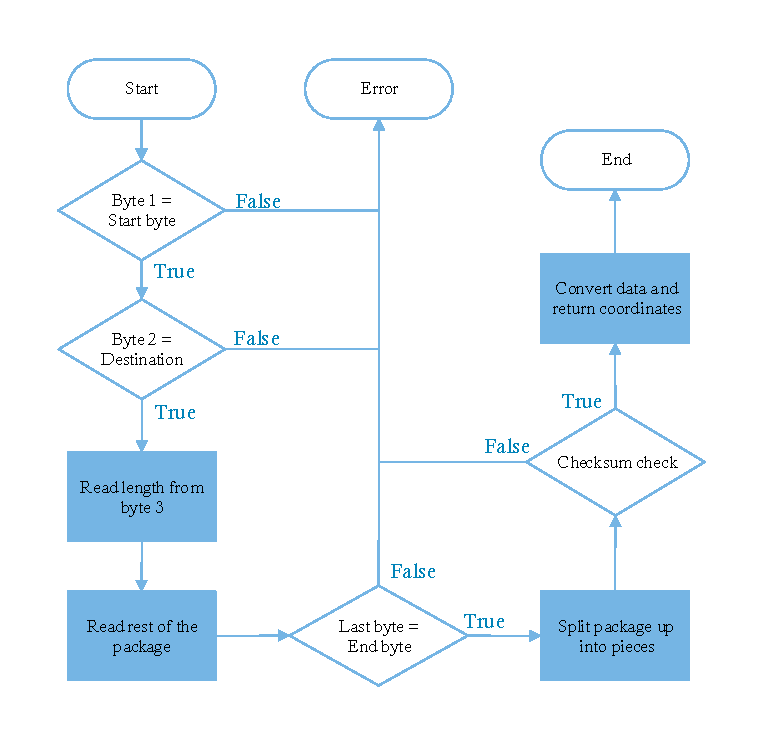
\includegraphics[scale=1.1]{figures/FlowReceiver.pdf}
\caption{Flow chart over the error handling in the receiver part.}
\label{FlowReceiver}
\end{figure}\vspace{-5mm}

If the package is transmitted correctly, the 1st byte received is the start byte and the 2nd byte is the destination ID of the receiver. The 3rd byte will contain 7 bit for the length and 1 bit for the first coordinate. If the length is without errors its value would be 96, which is 12 bytes. The last byte, the 12th one, is the end byte. If these condition are all correct, the receiver will check for errors utilizing the checksum. If that checksum is also correct, the system will convert the data and return the coordinates to the rest of the system.

If an error occurs, then all the bytes that have been read will be thrown away. Thus throwing the whole package away even if the start byte and the destination are correct, but the end byte is not. If the start byte is not correct, then only that byte will be thrown away until finding a correct start byte. This method is applied to ensure the system only utilizes complete packages.

This prevents the receiver to start in the middle of a package, as the system will throw away incomplete or damaged packages, until it finds a start byte. One example when utilizing this feature can cause a problem. If a start byte has a identical value with a byte in data or checksum. The problem will occur if the second byte is equal to the receivers destination ID, and the first seven bits of the next byte are equal to 96, which is the value of the length. An example on a situation where this problem occurs is illustrated in \tableref{errorPro}.

\begin{table}[H]
\centering
\begin{tabular}{c | m{0.1cm} m{0.1cm} m{0.1cm} m{0.1cm} m{0.1cm} m{0.1cm} m{0.1cm} m{0.1cm} | c | m{0.1cm} m{0.1cm} m{0.1cm} m{0.1cm} m{0.1cm} m{0.1cm} m{0.1cm} m{0.1cm} | l }
\multicolumn{9}{c}{Normal reading} & \multicolumn{9}{c}{Displaced reading} &  \\
\cline{2-9} \cline{11-18}
1st byte & 0 & 0 & 0 & 0 & 1 & 1 & 1 & 1 & 5th byte & 0 & 0 & 0 & 0 & 1 & 1 & 1 & 1 & $\leftarrow$ Start byte \\
\cline{2-9} \cline{11-18}
2nd byte & 0 & 0 & 0 & 0 & 0 & 0 & 0 & 1 & 6th byte & 0 & 0 & 0 & 0 & 0 & 0 & 0 & 1 & $\leftarrow$ Destination \\
\cline{2-9} \cline{11-18}
3rd byte & 0 & 0 & 0 & 0 & 0 & 1 & 1 & 0 & 7th byte & 0 & 0 & 0 & 0 & 0 & 1 & 1 & 0 & $\leftarrow$ Length (First seven bit)\\
\cline{2-9} \cline{11-18}
4th byte & 1 & 1 & 1 & 1 & 0 & 0 & 0 & 0 & 8th byte & 0 & 1 & 1 & 1 & 0 & 0 & 1 & 1 & \\
\cline{2-9} \cline{11-18}
5th byte & 0 & 0 & 0 & 0 & 1 & 1 & 1 & 1 & 9th byte & 1 & 0 & 0 & 1 & 1 & 0 & 1 & 1 & \\
\cline{2-9} \cline{11-18}
6th byte & 0 & 0 & 0 & 0 & 0 & 0 & 0 & 1 & 10th byte & 1 & 0 & 0 & 0 & 0 & 1 & 0 & 0 & \\
\cline{2-9} \cline{11-18}
7th byte & 0 & 0 & 0 & 0 & 0 & 1 & 1 & 0 & 11th byte & 0 & 0 & 1 & 1 & 0 & 1 & 1 & 1 & \\
\cline{2-9} \cline{11-18}
8th byte & 0 & 1 & 1 & 1 & 0 & 0 & 1 & 1 & 12th byte & 1 & 1 & 1 & 1 & 0 & 0 & 0 & 0 & \\
\cline{2-9} \cline{11-18}
9th byte & 1 & 0 & 0 & 1 & 1 & 0 & 1 & 1 & 1st byte & 0 & 0 & 0 & 0 & 1 & 1 & 1 & 1 & \\
\cline{2-9} \cline{11-18}
10th byte & 1 & 0 & 0 & 0 & 0 & 1 & 0 & 0 & 2nd byte & 0 & 0 & 0 & 0 & 0 & 0 & 0 & 1 & \\
\cline{2-9} \cline{11-18}
11th byte & 0 & 0 & 1 & 1 & 0 & 1 & 1 & 1 & 3rd byte & 0 & 0 & 0 & 0 & 0 & 1 & 1 & 0 & \\
\cline{2-9} \cline{11-18}
12th byte & 1 & 1 & 1 & 1 & 0 & 0 & 0 & 0 & 4th byte & 1 & 1 & 1 & 1 & 0 & 0 & 0 & 0 & $\leftarrow$ End byte\\
\cline{2-9} \cline{11-18}
\end{tabular}
\caption{Example of a normal reading of a package and a displaced reading of a package. The package contains the coordinates (-8222, 515, -3699).}
\label{errorPro}
\end{table}

In the example illustrated in \tableref{errorPro}, the 5th to 7th byte are equal to the start byte and the header. If the system is searching for the start byte and finds the 5th byte, it will begin to search for the header. In this case it will find it and as the 12th byte, which is in the next package, is equal to the end byte, the system will confirm it as a complete package. But since a checksum is implemented, it will be unlikely if the package is confirmed. The checksum, in this case, will not be the original checksum for the package, but another part of the package. As this checksum is not calculated to fit, the likelihood for the check going through is so poor, that error handling detecting this is not implemented. 

If a erroneous package is being stopped by the checksum, the 12 bytes would still have been read and is therefore thrown away. In the 12 bytes thrown away a correct start byte can be located. A problem can occur if the next three bytes, after the 12 bytes which is thrown away, is equal to the start byte and header again. Then the same scenario will repeat it self and will continue, until the three byte no longer equals the start byte and header. The scenario is unlikely, as three bytes has to be identical to the start byte and the header. 

The transport layer protocol implemented on top of the Xbee modules has now been described.

